\documentclass{article}
\usepackage[dvipdfmx]{graphicx}
\usepackage{parskip}
\usepackage{ascmac}
\usepackage{amsmath,amssymb}
\usepackage{cleveref}
    \crefname{proposition}{命題}{命題}
    \crefname{theorem}{定理}{定理}
    \crefname{lemma}{補題}{補題}
    \crefmultiformat{lemma}{補題~#2#1#3}{,~#2#1#3}{, #2#1#3}{,~#2#1#3}
\usepackage{autonum}
\usepackage{amsthm}
    \makeatletter
    \renewenvironment{proof}[1][\proofname]{\par
        \pushQED{\qed}
        \normalfont
        \topsep6\p@\@plus6\p@ \trivlist
        \item[\hskip\labelsep{\bfseries #1}\@addpunct{\bfseries}]\ignorespaces
    }{%
        \popQED\endtrivlist\@endpefalse
    }
    \renewcommand{\proofname}{証明.}
    \makeatother
\newtheorem{proposition}{命題}
\newtheorem{theorem}{定理}
\newtheorem{lemma}{補題}
\newcommand{\myparagraph}[1]{\paragraph{#1}\mbox{}\\}
\newcommand{\combination}[2]{{}_{#1} \mathrm{C}_{#2}}

\begin{document}

容器の体積を$V_0 = a^2b$とおく。
水がちょうど溢れるとき,容器内の水の形は四角柱(\cref{fig1})または三角柱(\cref{fig2})であり,
このときの水の体積は,
\begin{equation}
    x =
    \begin{cases}
        \vspace{15pt}
        a^2b - \dfrac{1}{2} a^3 \tan \theta & (x \geq \dfrac{1}{2} V_0\ \mbox{のとき}) \\
        \dfrac{ab^2}{2 \tan \theta} & (x < \dfrac{1}{2} V_0\ \mbox{のとき})
    \end{cases}
\end{equation}
と表せる。したがって,
\begin{equation}
    \theta =
    \begin{cases}
        \vspace{15pt}
        \arctan \dfrac{2 (a^2b - x)}{a^3} & (x \geq \dfrac{1}{2} V_0\ \mbox{のとき}) \\
        \arctan \dfrac{ab^2}{2x} & (x < \dfrac{1}{2} V_0\ \mbox{のとき})
    \end{cases}
\end{equation}
である。求める値は$\theta$を度数法に変換したものである。

\begin{figure}[h]
    \begin{center}
        \begin{tabular}{c}
            \begin{minipage}{0.45\hsize}
                \begin{center}
                    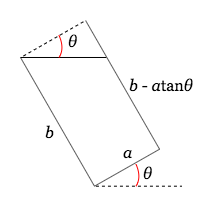
\includegraphics[width=140pt]{fig1.png}
                    \caption{四角柱}
                    \label{fig1}
                \end{center}
            \end{minipage}

            \begin{minipage}{0.45\hsize}
                \begin{center}
                    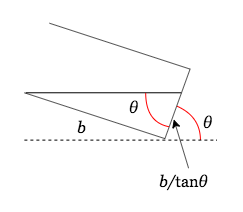
\includegraphics[width=140pt]{fig2.png}
                    \caption{三角柱}
                    \label{fig2}
                \end{center}
            \end{minipage}
        \end{tabular}
    \end{center}
\end{figure}

\end{document}
